\documentclass[a4paper,11pt]{article}

% Package imports
\usepackage{amsmath, amssymb, amsthm}
\usepackage{graphicx}
\usepackage{fancyhdr}
\usepackage{geometry}
\usepackage{titlesec}
\usepackage[nolist]{acronym}
\usepackage[most]{tcolorbox}

% Page layout
\geometry{left=2cm, right=2cm, top=2.5cm, bottom=2.5cm}
\graphicspath{ {./images/} }

% Header definition
\pagestyle{fancy}
\fancyhf{}
\lhead{Deep Learning Summary - WS24/25}
\rhead{\thepage}

% Theorem and definition styles with rounded borders and numbering
\newtcolorbox{definitionbox}{colback=white, colframe=black, arc=5pt, boxrule=1pt, left=5pt, right=5pt, top=5pt, bottom=5pt}
\newtcolorbox{theorembox}{colback=white, colframe=blue, arc=5pt, boxrule=1pt, left=5pt, right=5pt, top=5pt, bottom=5pt}

% Custom commands for numbered definitions and theorems
\newcounter{definitioncounter}
\newcounter{theoremcounter}

\setlength{\parindent}{0pt}
\setlength{\skip\footins}{0.5cm} % Adjust this to change the space above the footnotes
\raggedbottom

\newcommand{\definition}[1]{%
    \refstepcounter{definitioncounter}%
    \begin{definitionbox}
    \textbf{Definition \thedefinitioncounter:}
    \vspace{0.2cm}\newline
    #1
    \end{definitionbox}
    \vspace{0.3cm}
}

\newcommand{\theorem}[1]{%
    \refstepcounter{theoremcounter}%
    \begin{theorembox}
    \textbf{Theorem \thetheoremcounter:}
    \vspace{0.2cm}\newline
    #1
    \end{theorembox}
    \vspace{0.3cm}
}

\newcommand{\cf}[1]{\[#1\]}
\newcommand{\f}[1]{${#1}$}
\renewcommand{\b}[1]{\textbf{#1}}
\renewcommand{\it}[1]{\textit{#1}}
\newcommand{\pL}{\f{\mathcal{L}}}
\newcommand{\fL}{\mathcal{L}}

\begin{document}

\begin{acronym}[AAAAAA]
    \acro{mlp}[MLP]{Multi-Layer-Perceptron}
    \acro{cnn}[CNN]{Convolutional Neural Network}
    \acro{rnn}[RNN]{Recurrent Neural Network}
    \acro{vae}[VAE]{Variational Auto-Encoder}
    \acro{gan}[GAN]{Generative Adversarial Network}
    \acro{bn}[BN]{Batch Normalization}
    \acro{ln}[LN]{Layer Normalization}
    \acro{ml}[ML]{Machine Learning}
    \acro{dl}[DL]{Deep Learning}
    \acro{hpo}[HPO]{Hyperparameter Optimization}
    \acro{bptt}[BPTT]{backpropagation through time}
    \acro{mse}[MSE]{Mean Squared Error}
    \acro{kl}[KL]{Kullback-Leibler}
    \acro{mle}[MLE]{Maximum Likelihood Estimation}
    \acro{relu}[ReLU]{Rectified Linear Unit}
    \acro{sgd}[SGD]{Stochastic Gradient Descent}
    \acro{lstm}[LSTM]{Long Short-Term Memory}
\end{acronym}

% Title section
\begin{center}
    {\huge Deep Learning - WS24/25 \par}
    \vspace{0.5cm}
    {\large Niklas Rodenbüsch \par}
    \vspace{0.5cm}
    {\large \today \par}
\end{center}
\vspace{0.5cm}

\section{Introduction}
\subsection{Representation Learning vs. \ac{dl}}

\definition{Representation Learning is a set of methods that allows a machine to be fed with \b{raw data} and to \b{automatically discover the representations} needed for detection/classification.\\

\ac{dl} is Representation Learning with multiple levels of representations, obtained by \b{composing simple but nonlinear modules}.}
In Deep Learning, features are learned from raw data in an \b{end-to-end} fashion.

\subsection{\ac{ml} Concepts}
\subsubsection{Linear Regression}
Linear regression is a supervised learning algorithm that models the relationship between a dependent variable \f{y} and one or more independent variables \f{x} using a linear function.\\

The objective in linear regression is to minimize the \b{\ac{mse}} loss, given by:
\cf{\fL_{MSE}(\hat{y}, y) = \frac{1}{2N} \sum_{i=1}^{N} (\hat{y}_i - y_i)^2,}
where \f{\hat{y}=h_{\theta}(x)} is the prediction of the model and \f{N} is the total number of datapoints in the dataset.

\subsection{Logistic Regression}
Logistic regression is a classification algorithm that estimates the probability of a binary outcome using a logistic function.\\

For logistic regression, the objective is to minimize the \b{binary cross-entropy} loss:

\cf{\fL_{BCE}(\hat{y}, y) = -\frac{1}{N} \sum_{i=1}^{N} y_i \log \hat{y}_i + (1 - y_i) \log (1 - \hat{y}_i),}
where \f{\hat{y}=h_{\theta}(x)=g(w^Tx)} with \f{g(z)=\sigma(z)=\frac{1}{1+e^{-z}}} (\f{g} is the \b{sigmoid} function).\footnote{The correct formulation of the loss functions would be \f{\fL(\theta)} or \f{\fL(w)}.} For the Multi-Class classification case, the loss generalizes to:
\cf{
    \fL_{CE}(\theta) = -\frac{1}{N} \sum_{n=1}^{N}\sum_{k=1}^{K} y_{kn} \log \hat{y}_k(x_n, \theta).
}


\subsubsection{Overfitting and Underfitting}
\definition{\b{Overfitting} occurs when a model memorizes the training data. This leads to poor generalization on unseen data (e.g. the validation/test set).\\

\b{Underfitting} on the other hand means, that the model is not able to capture the complexity of the training data (e.g. because the model is too small).}

\subsubsection{Cross-Validation}
Cross-validation is a technique for assessing the performance of a model by dividing the dataset into multiple subsets, training the model on some subsets and testing it on others to ensure it generalizes well to unseen data.

\subsection{Basics of Neural Networks}
\subsubsection{Types of Tasks}
\begin{itemize}
    \item \b{Possible Inputs:} Sound, Text, Images, Graphs
    \item \b{Possible Outputs:} Classification, Regression, Sound, Text, Images, ... 
\end{itemize}

\subsubsection{Single Neurons}
A neuron in a neural network computes the \b{weighted sum \f{z} of its inputs \f{x}} and performs a \b{nonlinear transformation} \f{h(z)} afterwards:
\cf{a = h(z)\quad,\quad z = x_1w_1 + x_2w_2+ ... + x_nw_n}

\section{\acp{mlp}}
\subsection{Entropy \& \ac{kl}-Divergence}
\definition{\b{Information entropy} quantifies the uncertainty about a random variable \f{X} (assume \f{X} has \f{K} possible outcomes):
\cf{H(P) = - \mathbb{E}_{x\sim P}\left[\log P(x)\right]}
\cf{H(P) = - \sum_{k=1}^{K}P(X=x_k)\log P(X=x_k)}}

\definition{Given a true probability distribution \( P \) and a predicted distribution \( Q \), the \b{Cross-Entropy} of the same random variable \f{X} is defined as:
\cf{H(P,Q) = - \mathbb{E}_{x\sim P}\left[\log Q(x)\right]}
\cf{H(P,Q) = - \sum_{k=1}^{K}P(x_k)\log Q(x_k)}}

\definition{\b{\ac{kl}-Divergence} is a measure of how one probability distribution \f{P} diverges from a second, expected probability distribution \f{Q}. The KL-divergence is defined as:
\cf{D_{\text{KL}}(P \parallel Q) = H(P,Q) - H(P) = -\mathbb{E}_{x\sim P}\left[\log \frac{Q(x)}{P(x)}\right]}
}
The \ac{kl}-Divergence can be interpreted as the \b{information loss if we use distribution Q to approximate distribution P.}

KL-Divergence is always non-negative, not symmetric and is zero if and only if \( P = Q \).

\subsection{\ac{mle}}
\ac{mle} is a method for estimating the parameters of a statistical model by maximizing the likelihood function, which represents the probability of observing the given data under various parameter values (in other words: the model "fitting" itself to match the observed data). The MLE is defined as:
\[
\theta_{\text{MLE}} = \arg\max_{\theta} p_{\text{model}}(\mathbb{X};\theta) = \arg\max_{\theta} \prod_{i=1}^{n} p(x_i \mid \theta)= \arg\max_{\theta} \sum_{i=1}^{n} \log p(x_i \mid \theta),
\]
where \f{\mathbb{X} = \{x_1, ..., x_n\}} is a set of \f{n} samples drawn from the unknown data-generating distribution \f{p_{\text{data}}}, and \( p_{\text{model}}(x_i \mid \theta) \) is the probability of observing the data point \( x_i \) given the parameters \( \theta \).


\subsection{\acl{mlp}}
The \ac{mlp} extends the simple Perceptron by adding (multiple) fully-connected hidden layers between the input and the output layer. The forward pass is computed the following way (assume the network has one hidden layer):
\cf{\hat{y} = g^{(2)}(W^{{(2)}^T}g^{(1)}(W^{{(1)}^T}x+b^{(1)})+b^{(2)})}
\b{Note:} The weight matrices in the first layer are of shape \f{(\text{dim\_x}\times \text{n\_neurons})^T}.
\theorem{The Universal Function Approximation Theorem states that:
\begin{enumerate}
\item \b{Any boolean function} can be realized by an MLP with one hidden layer.
\item \b{Any bounded continouos function} can be approximated with arbitrary precision by a MLP with one hidden layer.
\end{enumerate}}
\b{Note:} The theorem does not show that any function can be learned from data!

\theorem{
    A neural network with \f{n_0} inputs and \f{K} layers of \f{n} units each, with \ac{relu} activations can represent functions that have \f{\Omega((\frac{n}{n_0})^{(K-1)n_0}n^{n_0})} linear regions.}


\subsection{Activation Functions}
\begin{itemize}
    \item \b{Linear:} \f{h_{\text{linear}}(z) = z}
    \item \b{Hyperbolic Tangent:} \f{h_{\text{tanh}}(z)=\text{tanh}(z)=\frac{\exp(z)-\exp(-z)}{\exp(z)+\exp(-z)}\in[-1;1]}
    \item \b{\ac{relu}:} \f{h_{\text{relu}}(z) = \max(0,z)}
    \item \b{Parametric ReLU (PReLU):} \f{h_{\text{relu}}(z)=\begin{cases} 
        z, & z>0 \\
        az, & z\leq 0
    \end{cases}}, where \f{a>0} is a learnable parameter.
    \item \b{Exponential Linear Unit (ELU):} \f{h_{\text{elu}}(z)=\begin{cases} 
        z, & z>0 \\
        \alpha(\exp(z)-1), & z\leq 0
    \end{cases}}, with \f{\alpha > 0}.
    \item \b{Gaussian Error Linear Unit (GELU):} \f{h_{\text{gelu}}(z) = z\phi(z)}, where \f{\phi} is the CDF.
    \item \b{Swish:} \f{h_{\text{swish}}(z)=z\sigma(\beta z)}, where \f{\beta \geq 0} is constant or a trainable parameter.
    \item \b{Softmax:} \f{h_{\text{softmax}}(z) = \frac{\exp(z)}{\sum_j\exp(z_j)} = p(y_j=1) \in [0;1]}, for MCC output layer
\end{itemize}

\section{Backpropagation}
\definition{The \b{chain rule} computes the derivatives for \b{compositions} of functions \f{g(x)} and \f{f(y)=f(g(x))=z} as:
\cf{
    (f\circ g)^\prime(x) = (f(g(x)))^\prime = f^\prime(g(x))\cdot g^\prime(x)
}
\cf{
    \frac{\delta z}{\delta x} = \frac{\delta z}{\delta y}\frac{\delta y}{\delta x} = \frac{\delta f(g(x))}{\delta g(x)}\frac{\delta g(x)}{\delta x}
}}

Generalizing this formulation to the multidimensional case with leads us to:

\cf{
    \frac{\delta z}{\delta x_i}=\sum_{j}^{}\frac{\delta z}{\delta y_j}\frac{\delta y_j}{\delta x_i}
}
where \f{x\in\mathbb{R}^m, y\in\mathbb{R}^n, g:\mathbb{R}^m\to\mathbb{R}^n, f:\mathbb{R}^n\to\mathbb{R}} and \f{y = g(x)} and \f{z = f(y)}. Transforming this formulation into vector notation gives us:
\cf{
    \nabla_{x}z=(\frac{\delta y}{\delta x})^T\nabla_yz,
}
where \f{\frac{\delta y}{\delta x}} is the \f{n\times m} Jacobian matrix of \f{g}, and \f{\nabla_yz} being the gradient of z with respect to vector \f{y}. Since \f{y \in \mathbb{R}^n} this leaves us with:
\cf{
    \nabla_yz=\left[ \frac{\delta z}{\delta y_1}, \frac{\delta z}{\delta y_2}, ..., \frac{\delta z}{\delta y_n} \right]^T
}

\subsection{Derivations of Activations}
\begin{itemize}
    \item \b{Linear:} \f{h^\prime(z)=1}
    \item \b{Sigmoid:} \f{h^\prime(z)=h(z)(1-h(z))}
    \item \b{Tanh:} \f{h^\prime(z)=1-h(z)^2}
    \item \b{ReLU:} \f{h^\prime(z)=\begin{cases}
        1, z>0\\
        0, z\leq0
    \end{cases}}
\end{itemize}

\subsection{Backpropagation in Neural Networks}
\vspace{0.3cm}
\begin{figure}[h]
    \centering
    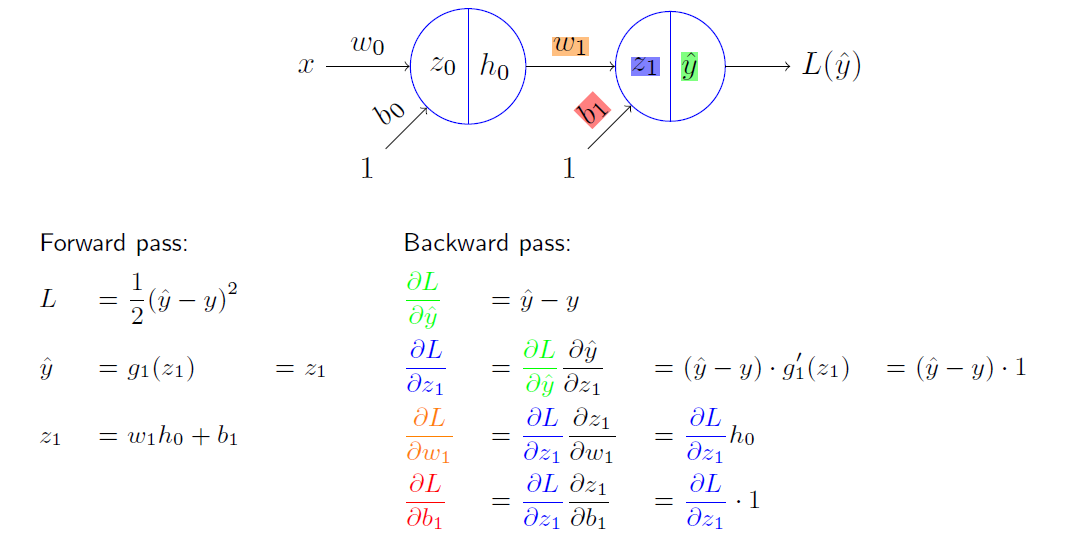
\includegraphics[width=0.9\textwidth]{bp1.png}
\end{figure}
\vspace{0.3cm}
\begin{figure}[h]
    \centering
    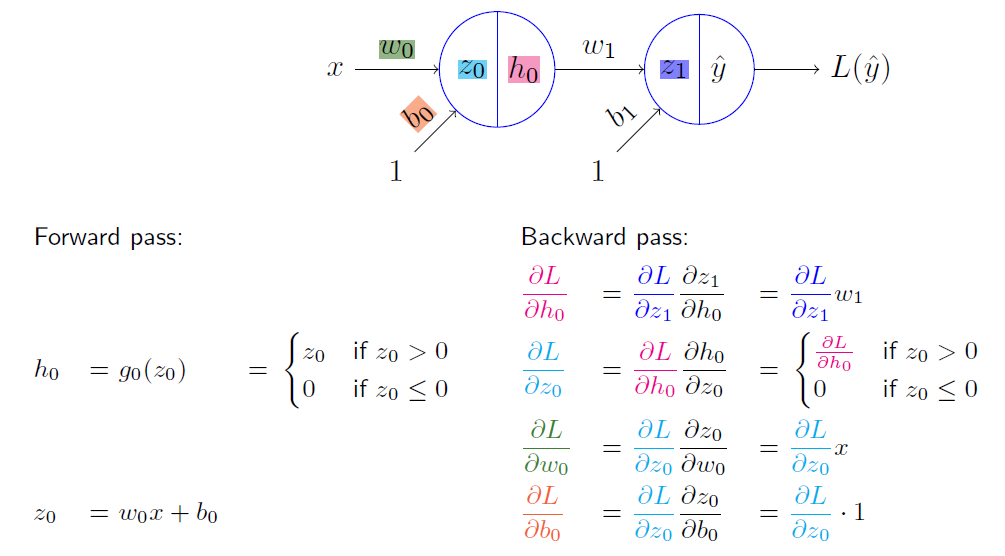
\includegraphics[width=0.9\textwidth]{bp2.png}
\end{figure}

\b{Note:} The gradient of a skip connection is computed by summing the incoming derivatives of both the forward and skip connection.

\section{Optimization}
\subsection{Optimization vs. Learning}

The goal of optimization in \ac{dl} is to maximize the performance on some measure P. Since P might be intractable (0/1 accuracy not differentiable), we introduce a surrogate loss function \pL, which is \b{tractable, differentiable} and \b{might enable better generalization}.\\
In practice, optimizing \f{\mathcal{L}} directly may not generalize well (overfitting). In order to mitigate this, we can add regularization terms to the loss function.

\definition{\b{Learning} in contrast is distinguished from pure optimization by the following points:
\begin{itemize}
    \item May have to use surrogate instead of the real objective such as softmax instead of hard-max.
    \item Optimization on partial data distribution instead of the real distribution.
    \item Often introduces regularization term to generalize.
    \item Requires the summation over given data points, so computationally expensive for a large dataset.
\end{itemize} }

\subsection{Gradient-Based Optimization}
In order to minimize the loss of the model, we need to find a global minimum of \pL. Even though this could be solved analytically (the gradient is \f{0} at a minimum), this is not feasible in practice. Instead, we use the numerical (iterative) method of \b{Gradient Descent}.\\
The algorithm is described in the following figure:
\vspace{0.3cm}
\begin{figure}[h]
    \centering
    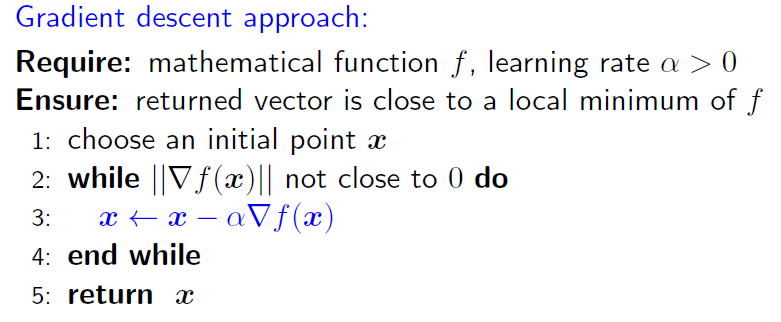
\includegraphics[width=0.6\textwidth]{gd.png}
\end{figure}

\subsection{Ill-Conditioning}
The condition number \f{\kappa(Q)} of a matrix \f{Q} with eigenvalues \f{\lambda} is defined as \f{\kappa(Q)=\frac{\lambda_{\max}}{\lambda_{\min}}}.\\
Matrices with large condition number are called \b{ill-conditioned}.\\
Ill-conditioned matrices drastically hurt convergence performance by causing \b{zig-zag behavior} (one dimension contributes more than the others)!\\[0.5em]

There are two methods to mitigate this issue in practice: \b{momentum} and \b{preconditioning}.

\definition{\b{Momentum} takes into account the direction of the previous gradients by adding an extrapolation step (\f{\beta}) to the gradient step:
\cf{
    x_{k+1}=x_k - \alpha\nabla f(x_k) + \beta(x_k - x_{k-1}) = x_k - \alpha\sum_{i=0}^{k}\beta^{k-i}g_i
}}

\definition{\b{Preconditioning} makes use of a \b{preconditioning matrix} \f{D_k} (positiv definite and symmetric) to pre-multiply the gradients by \f{D_k} in order to scale the gradients:
\cf{
    x_{k+1} = x_k - \alpha D_k \nabla f(x_k)
}
\b{Note:} The best scaling is the inverse of the Hessian matrix \f{D_k = \nabla^2f(x_k)^{-1}} (Newton's method). The problem with Newton's method is that it is also attracted to maximizers.}

\subsection{Challenges of Optimization}
\begin{itemize}
    \item \b{Non-Convexity:} The model m is a highly non-convex function (saddle points very likely).
    \item \b{Large datasets:} In modern datasets, \f{N} is large (makes gradient calculation very expensive).
    \item \b{High dimensionality:} In modern neural networks, \f{d} is very large.
    \item \b{Structure of the network:} Can yield hard-to-optimize response surfaces.
\end{itemize}
Furthermore, the following properties in the structure of neural networks make optimizations harder:
\begin{enumerate}
    \item \b{Cliff-like surfaces in the searching space:} he gradients suddenly drop or rise signifcantly at some points, especially in \acp{rnn}.
    \item \b{Gradient vanishing and exploding:} Since we have to multiply matrices again and again, each value is going to be very small or large by the power factor.
\end{enumerate}

\subsection{\ac{sgd}}
While standard gradient descent handles learning by epoch, SGD computes the loss value using only a part of the dataset. Note that learning by epoch is to learn all the training data at the same time. Typically, the optimization by gradient descent is stable, but it takes a lot more time. Therefore, we use so-called \b{mini-batches}, i.e. a part of the dataset, for one update step. SGD stochastically picks a batch of data points and learns the batch at each step.\\
SGD is preferred due to the following reasons:

\begin{enumerate}
    \item Much quicker training allows much more iterations.
    \item Since the standard error of empirical loss function against true loss function decreases by the order of \f{O(\frac{1}{\sqrt{B}})} where \f{B} is the batch size, a larger batch size does not make a big difference.
    \item The training dataset can include many similar data points, so mini-batch learning is likely to yield similar results to that of full-set training.
    \item Since mini-batch includes less data points and the standard error is larger, the neural networks are not likely to overfit the statistics of the given data distribution.
\end{enumerate}

\b{Note:} We typically want to set the batch size as large as possible given memory constraints. However, small batch sizes can have a regularizing effect (small batch size requires lower learning rates). In order to mitigate biases of the data collection process, we randomly shuffle the training data before drawing batches.

\subsection{Learning Rate Schedules}
Setting the learning rate \f{\alpha} correctly is very important for good model convergence. Too low a learning rate can drastically slow down convergence, while too high a learning rate might lead to divergence.\\[0.5em]
Generally, using a fixed learning rate is not a good practice, as SGD would never converge. For this reason, dynamic learning rate scheduling is used:
\begin{itemize}
    \item \b{Linear decay:} Until iteration \f{\tau}: \f{\alpha_k = (1-b)\alpha_0 + b\alpha_\tau,} with \f{b=k/\tau}. Then constant.
    \item \b{Exponential decay:} \f{\alpha_k = b\alpha_{k-1}=b^k\alpha_0}
    \item \b{Step decay:} Decay by a factor (e.g. 10) every n steps.
    \item \b{Cosine decay:} \f{\alpha_k = \frac{1}{2}(1+\cos(\frac{k}{n}\pi))\times \alpha_0}, with \f{n} being the total number of epochs.
    \item \b{SGD with warm restarts (SGDR):} Consists of multiple repeated steps
    \begin{enumerate}
        \item Quickly cool down \f{\alpha} to zero
        \item Heat up \f{\alpha} again
        \item Cool down \f{\alpha} more slowly.
    \end{enumerate}
\end{itemize}

\subsection{SGD with Momentum}
As introduced before, momentum \f{v} (velocity) is an exponentially moving average of past gradients. This makes updates smoother by keeping a history. Update step:
\cf{v \leftarrow \beta v - \alpha \hat{g}}
\cf{\theta \leftarrow \theta + v}
Advantages of using momentum are:
\begin{itemize}
    \item Smoothes zig-zagging
    \item Accelerates learning at flat spots
    \item Slows down when signs of partial derivatives change
\end{itemize}
\b{Disadvantages}: additional parameter \f{\beta}, strong momentum might cause more zig-zagging

\subsection{Adaptive Gradient Algorithms}
The learning rate has to be adapted for convergence. However, to do so may require different learning rates for different dimensions. This is where adaptive gradient algorithms come into play:
\begin{enumerate}
    \item \b{AdaGrad:} Update step:
    \begin{enumerate}
        \item \f{r \leftarrow r + \hat{g} \odot \hat{g}\quad} (accumulate squared gradient)
        \item \f{\Delta\theta \leftarrow - \frac{\alpha}{\epsilon + \sqrt{r}} \odot \hat{g}\quad} (scale \f{\alpha} by root of cumulative squared gradient, \f{\epsilon << 1})
        \item \f{\theta \leftarrow \theta + \Delta\theta\quad} (update model weights)
    \end{enumerate}
    \begin{itemize}
        \item High learning rate for dimensions with small gradient.
        \item Sometimes decreases learning rate too early due to long influences of past gradients.
    \end{itemize}
    \item \b{RMSProp:} Update step:
    \begin{enumerate}
        \item \f{r \leftarrow \rho r + (1-\rho)\hat{g} \odot \hat{g}\quad} (EMA of squared gradient)
        \item \f{\Delta\theta \leftarrow - \frac{\alpha}{\epsilon + \sqrt{r}} \odot \hat{g}\quad}
        \item \f{\theta \leftarrow \theta + \Delta\theta\quad}
    \end{enumerate}
    \begin{itemize}
        \item \f{\rho} is a new hyperparameter controlling how quickly past gradients are forgotten.
    \end{itemize}
    \item \b{Adam:} Update step:
    \begin{enumerate}
        \item \f{t \leftarrow t + 1}
        \item \f{s \leftarrow \rho_1s + (1-\rho_1)\hat{g}\quad} (EMA of gradient)
        \item \f{r \leftarrow \rho_2r + (1-\rho_2)\hat{g} \odot \hat{g}\quad} (EMA of squared gradient)
        \item \f{\hat{s} \leftarrow \frac{s}{1-\rho_1^t}\quad} (correct bias in moving gradient estimate)
        \item \f{\hat{r} \leftarrow \frac{r}{1-\rho_2^t}\quad} (correct bias in sq. moving bias estimate)
        \item \f{\Delta\theta \leftarrow - \frac{\alpha}{\epsilon + \sqrt{\hat{r}}} \odot \hat{s}\quad}
        \item \f{\theta \leftarrow \theta + \Delta\theta\quad}
    \end{enumerate}
    \begin{itemize}
        \item \f{\rho_i} are decay rates for first and second moment.
        \item Extension of RMSProp with momentum and bias correction.
    \end{itemize}
\end{enumerate}

\section{Regularization}
Usually deep neural networks habe low bias and high variance (meaning that if you change the training data a little the fitted function may change a lot). The standard bias-variance tradeoff is defined by:
\cf{\text{expected loss} = (\text{bias})^2+\text{variance}+\text{noise}}
\b{The goal of regularization is to introduce \it{some} bias, to substantially reduce variance and therefore to lower the generalization loss.}

\definition{\b{Early Stopping} stops the training when the error on the validation set has reached its minimum (i.e. as soon as it starts to increase again). The disadvantage is that this need perpetual oberservation of the error.}

\subsection{Small Weights (Shrinkage Methods)}
Idea: Extend the loss function with an extra \b{regularizer} (penalty) term of strength \f{\lambda} to prevent overfitting:
\cf{
    \fL(\theta) = \fL_D(\theta) + \lambda\fL_{reg}(\theta)
}
\cf{
    \fL_{reg}(\theta) = \frac{1}{q}\sum_{j=1}^{M}|\theta_j|^q \quad \to \quad \begin{cases}
        q=1: L_1 \text{ regularizer (lasso)}\\
        q=2: L_2 \text{ regularizer (ridge)}
    \end{cases}
}

\subsection{Decoupled Weight Decay}
\f{L_2} regularization is typically implemented by directly changing the gradient to:
\cf{g^\prime = g + \lambda\theta,}
and thus changing the SGD update to:
\cf{
    \theta \leftarrow \theta- \alpha g^\prime = (1-\alpha\lambda)\theta - \alpha g
}
\b{Decoupled Weight Decay} pulls the weights towards zero at each update step of SGD (note that for \f{\lambda = w/\alpha} this is equivalent to \f{L_2}):
\cf{\theta\leftarrow(1-w)\theta-\alpha g}
The difference to \f{L_2} is that in \f{L_2} the hyperparameters \f{\lambda} and \f{\alpha} are coupled!\\
Decoupled weight decay gave rise to the popular \b{AdamW} algorithm, which is essentially Adam combined with weight decay.

\subsection{Parameter Sharing/Tying}
Idea: Sharing parameters across the network. This is, e.g., used in \acp{cnn} where the same filters are used across the input image, which makes feature detection invariant to translations. It is also used in \acp{rnn} where the same network is applied at each time step.\\
Sharing the parameters \b{controls the networks capacity}, \b{encourages the search for regular patterns} and \b{limits memory cost}.
\definition{Parameter sharing is e.g. applied in \b{multitask learning}, where one network is used to tackle multiple tasks at once by an intermediate shared layer and individual models branching off of it. If the tasks are related, this can have a similar effect as additional training data.}
\b{Parameter tying} allows models to be similar to each other, by adding a soft constraints to the parameters of each model. If the tasks are similar, this can be done by for example leveraging the \f{L_2} regularization:
\cf{
    \Omega(\theta^{(A)}, \theta^{(B)}) = \Vert \theta^{(A)} - \theta^{(B)}\Vert_2^2
}

\subsection{Dropout}
\b{Dropout} randomly drops units from the network during training by multiplying their output by zero with a probability of \f{p}. For each datapoint a different dropout mask is sampled. This avoids co-adaption of the weights (reliance on previous units). It is important to note that we have to store the location of dropped weights in the forward pass to ignore the update in the backward pass.\\[0.5em]

Applying dropout can be seen as training an ensemble of \f{2^n} networks with shared weights, where \f{n} is the number of dropped units.

\subsection{Data Augmentation}
Data augmentation is used to increase the data amount by applying some simple transformation to a training dataset and adding this transformed data to the training dataset.\\[0.5em]
Possible transformations: \b{translation, scaling, reflection, rotation, stretching}\\
Domain-Specific: replacing words with synonyms, adding background noise, change speed\\

Note that since CNNs have invariance with respect to the movement along each axis, trans-
lation does not make sense. The drawback of data augmentation is to require more computational time proportional to the data size. Additionally, the improvement diminishes as the augmented amount increases.\\

There exist several techniques to find suitable augmentations automatically:
\begin{enumerate}
    \item \b{AutoAugment:} Search for best augmentation combinations automatically, large comp. cost.
    \item \b{RandAugment:} Randomly sample \f{N} augmentations with strength \f{M}, similar results as AutoAugment but much cheaper.
    \item \b{TrivialAugment:} Randomly sample one augmentation and \f{M} for each image in a batch.
\end{enumerate}

\subsection{Noise Robustness}
Goal: Improving robustness by training with randomly added noise. Note that data augmentations are the noise added to the inputs. Noise can be added in several more places:
\begin{itemize}
    \item Hidden Units: Data augmentation at various levels of abstractness
    \item Weights: Stochastic implementation of Bayesian inference
    \item Outputs: Label smoothing
\end{itemize}

\subsection{Adversarial Training}
Adversarial data is data which can decept a trained model. The procedure for adversarial training is as follows:
\begin{enumerate}
    \item Train network on training examples.
    \item Generate adversarial examples for this network.
    \item Add adversarial examples to training data and repeat.
\end{enumerate}


\subsection{Ensemble Methods}
\begin{itemize}
    \item \b{Bagging:}
    \begin{enumerate}
        \item Randomly draw data with "zurücklegen" for each model
        \item Aggregate the output of all trained models in an ensemble classifier
        \item[\f{=>}] Introduces bias but reduces variance
    \end{enumerate} 
    \item \b{Deep Ensembles:}
    \begin{enumerate}
        \item Train several deep networks on the same data, rely on SGD to find different minima
        \item Aggregate the output of all models (e.g. by averaging)
        \item[\f{=>}] Does not introduce bias, but reduces variance
        \item[\f{=>}] \f{k}-fold increase in complexity of all types (\f{k} models)
    \end{enumerate}
    \item \b{Hyperdeep Ensembles:}
    \begin{enumerate}
        \item Train using SGD with weight restarts
        \item Take snapshots of weights before each restart and ensemble them 
        \item[\f{=>}] Reduces time complexity to a single training run
    \end{enumerate}
\end{itemize}

\section{\acp{cnn}}
\acp{cnn} are specially structured neural networks that are very well suited to process grid-like data such as images and time series. They make use of convolutional layers, which perform a \b{convolution operation} followed by some nonlinearity and \b{pooling}.

\definition{The \b{operation of convolution} works by sliding a kernel/filter over the input and computing the dot products, thus reducing dimensionality and resulting in the so called "activation map" (one for each filter). Note that the filter always matches the depth channel of the input data. Convolutions are defined as:
\cf{
    S(i,j)=(K*I)(i,j)=\sum_{m}^{}\sum_{n}^{}I(i-m,j-n)K(m,n)
}
Note that convolutions and cross-correlation are similar. Flipping the kernel by 180° and applying cross-correlation is equal to convolution.}

\subsection{More Properties of Convolutions}
In order to \b{keep the spatial dimension} after applying convolution, typically we see Convolutional layers with stride 1, \f{F\times F} filters and zero padding with \f{(F-1/2)} pixels.\\

\b{Valid Convolution:} When no padding is applied and the kernel is fully contained within the image.\\

\b{Same Convolution:} Applying padding to keep the image dimension constant.\\

With an input of shape \f{W_1\times H_1\times D_1}, the size of the convolution output \f{W_2\times H_2\times D_2} is given by:
\cf{W_2 = (W_1 - F + 2P)/S+1}
\cf{H_2 = (H_1 - F + 2P)/S+1}
\cf{D_2 = K}

\vspace{0.5em}
Using filters of size \f{F\times F\times D_1} and enabling parameter sharing, convolutions introduce \f{(FFD_1)K} weights and \f{K} biases.\\

Convolution leverages three important ideas:
\begin{itemize}
    \item Sparse interactions (if kernel \f{<} input) \f{\to} Receptive field increases with depth
    \item Parameter sharing
    \item Equivariant Representations: Change of input leads to same change of output
\end{itemize}

\subsection{Miscellaneous Convolutions}
\begin{enumerate}
    \item \b{3D-Convolutions:} The filter can move in all three directions and the filter depth should be smaller than the input layer depth (i.e. kernel depth \f{<} channel size). Useful for data such as videos or MRI images.
    \item \b{\f{1\times 1} Convolution:} Also called feature pooling, reduces dimensionality for efficient computations to \f{W\times H\times 1}. Enables more complex representations using non-linearity.
    \item \b{Transposed Convolution:} This convolution up-samples data by combining the padding and convolution.
    \item \b{Dilated Convolution:} It in ates the kernel by inserting spaces between kernel elements while keeping the kernel size; therefore no additional cost is required. Since it convolutes elements from a larger range, we can often get much larger receptive field.
    \item \b{Grouped Convolution:} Filters at each layer are separated into certain numbers of groups and each group is responsible for convolutions of the corresponding group. The advantage of this convolution is efficient training.
    \item \b{Spacially Separable convolutions:} It first convolutes only along one axis and then it convolutes the convoluted data along the other axis in two separate steps. The adavantages of this convolution are less parameters and less matrix multiplications. On the other hand, training results can be suboptimal.
    \item \b{Depthwise Separable Convolutions:} It first convolutes each channel separately, and then it applies \f{1\times 1} convolution to the data. This convolution also yields the same benefits and problems as spatially separable convolutions.
\end{enumerate}

\subsection{Pooling}
\b{Pooling layers} (separately) reduce the size of the activation maps (downsampling) with the effect of making representations approximately invariant to small input translations.\\
One popular choice, namely \b{max-pooling} selects the maximum value in the area of the filter.\\
The formulas for the output size are the same as for convolutional layers, but without padding.

\section{\acp{rnn}}
\subsection{General}
\acp{rnn} allow for cycles in the connectivity graph. These cycles allow information to persist in the network for some time (state) and provide a fading memory. This makes \acp{rnn} extremely powerful at processing sequences. \b{\acp{rnn} are Turing-complete and can represent dynamical systems rather than function mappings.}\\
There are several ways to use \acp{rnn}:
\begin{itemize}
    \item \b{One-to-many:} Image caption generation.
    \item \b{Many-to-one:} Giving a numerical score to a given review.
    \item \b{Many-to-many:} Video frame classification, language translation.
\end{itemize}

\subsection{Design Patterns}
\acp{rnn} produce outputs at every step \f{t}, with recurrent connections between hidden units. The unfolded network can be seen in the figure below. \acp{rnn} are trained with \ac{bptt}, which is backpropagation with weight sharing over the unrolled computational graph.\\
The forward pass is defined the following:
\cf{h^{(t)} = \tanh(Wh^{(t-1)}+Ux^{(t)} + b)}
\cf{\hat{y}^{(t)}=\text{softmax}(o^{(t)})=\text{softmax}(c+Vh^{(t)}),}
where \f{W,U,V} are shared weight matrices of the hidden units and \f{b,c} are shared bias vectors for the hidden states and outputs respectively.\\[0.5em]

\begin{figure}[ht]
    \centering
    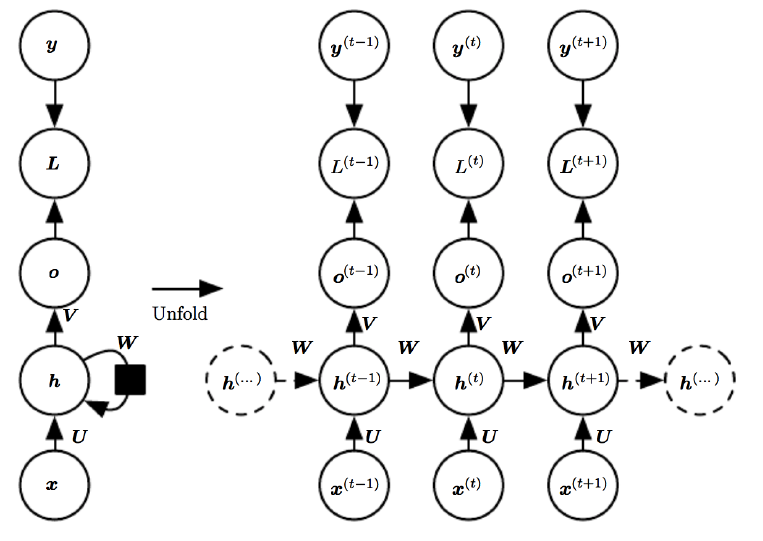
\includegraphics[width=0.5\textwidth]{rnn.png}
\end{figure}


An alternative to having the recurrent connections between the hidden units, is having them go \b{from the output to the successive hidden unit}. Even though this is potentially less powerful, it has the advantage that it can be trained with \b{teacher forcing}.\\
Here, during training time, the hidden layers are fed with the true label of the previous step instead of the models own prediction. This enables the model to learn from the data directly, but it approximates based on the predictions during test time which makes it likely to accumulate errors over time.

\subsection{Miscellaneous Architectures}
\begin{enumerate}
    \item \b{Many-to-One:} Recurrent connections etween hidden units, output only at last step (BPTT).
    \item \b{One-to-Many:} Mapping static input into distribution over sequences of \f{y}. Outputs at every step.
    \item \b{Many-to-Many:} Mapping variable length sequence of inputs into distribution over sequences of \f{y}. Can be combined with teacher forcing and \ac{bptt}.
\end{enumerate}

Additional architectures: \b{Bidirectional \ac{rnn}} with two directional hidden states can use information from both past and future. Since it requires future information, it cannot be used for online tasks. \b{Encoder-Decoder seq.-to-seq.} architecture are used when the length of inputs and outputs are different, such as for translation.

\subsection{Problems during Training}
Although RNNs have powerful non-linear processing due to the repeating application of the same function, it also induces some problems. Typical problems are gradient vanishing and explosion. The solution for the explosion is gradient clipping and that for the vanishing is the LSTM.

\subsection{Truncated BPTT}
BPTT is expensive and possibly unstable. Furthermore it can lead to vanishing/exploding gradients. The solution is to use truncated BPTT, which truncates gradients after fixed intervals (often aligned with batch-size). Requires sequential data loading. 

\subsection{\ac{lstm}}
The LSTM was introduced to address the vanishing gradient problem. Its architecture consists of special memory cells with \b{forget, input} and \b{outpus gates}. By now the LSTM has become the standard RNN model in many applications.\\[0.3em]

\begin{figure}[ht]
    \centering
    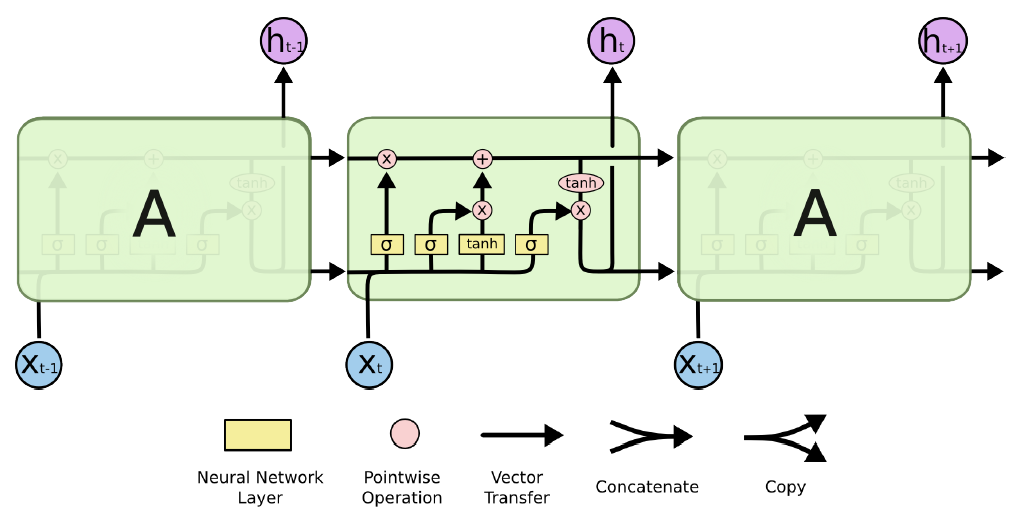
\includegraphics[width=0.7\textwidth]{lstm.png}
\end{figure}

Since this model has a self-loop of inner state \f{C} without any activations, the gradient with respect to \f{C} does not vanish nearly as RNNs do. The forget gate decays less important features from the past and maintain important features. The input gate takes two vectors \f{i_t} and \f{\tilde{c_t}} and controls how much new information we should store and in which direction we should change the state. The output gate controls which features to use. The advantages of LSTM are that it can selectively forget and remember features and each parameter of LSTM already have their meanings.

\section{Attention \& Transformers}
\subsection{Types of Attention}
\begin{itemize}
    \item \b{Implicit Attention:} A trained neural network reacts more strongly to some parts of the input than to others. This can be quantified by calculating the gradient of a class output w.r.t the input pixels to create an attention map.
    \item \b{Explicit Attention:} These mechanisms actively focus on parts of the input data (and downweight others). Here, the network computes input-dependent attention weights (example: LSTM input gate).
\end{itemize}

\subsection{RNNs with Attention}
\b{Encoder-Decoder Networks:} The encoder processes the input sequence into a context vector. The decoder then takes the context vector and produces the output sequence. The context vector is usually the last hidden state of the encoder. Here the disadvantage lays in the fact that one vector has to encode the information for all inputs.\\

\b{Idea:} What if we were to pass all encoder hidden states to the decoder which then learns to focus on relevant parts?\\

\b{Decoder-Attention:} The decoder computes scores for each of the hidden states it received and thus "attends" to the relevant hidden states during each decoding step. Each hidden state is multiplied by it soft-maxed score. The scores are computed using a feedforward neural network.

\subsection{Transformers}
In contrast to \acp{rnn}, Transformers can handle all inputs in one single step. From a high-level overview, the architecture simply consists of a couple stacked encoder blocks followed by a couple stacked decoder blocks.\\[0.1em]

Each \b{encoder block} consists of a self-attention layer followed by a fully connected layer.\\

Each \b{decoder block} consists of a self-attention layer followed by an encoder-decoder attention layer and a fully connected layer.

\subsection{Encoder: Flow of Vectors}
In the encoder, each input word get encoded into a fixed-sized vector of size \f{d}. The self-attention blocks operate on all inputs jointly, while the FC layers operate on each word separately. Throughout the encoder block, the representation of each word gets transformed to consider the entire sentence.

\subsection{Self-Attention}
Attention can be seen as sort of a soft retrieval from a database. Given a list of key-value pairs stored in the database and a query \f{q}, attention compares \f{q} to the keys and returns the weighted average of the values:
\cf{
    \text{attention}(q,k,v) = \sum_{i=1}^{N}\text{softmax}(\text{Similarity}(q,k_i))\times v_i
}
There are several popular ways to compute the similarity score:
\begin{itemize}
    \item \b{Dot-Product:} \f{q^Tk_i}
    \item \b{Scaled-Dot-Product:} \f{\frac{q^Tk_i}{\sqrt{d}},\quad} with \f{d} being the dimensionality of the keys, used in Transformers
    \item \b{Generalized Dot-Product:} \f{g^TWk_i}
    \item \b{Additive similarity:} \f{w_q^Tq+w_k^Tk_i}
\end{itemize}
\b{Important:} In self-attention, queries, keys and values are all derived from the same input sequence! For each input \f{x_i} we compute query \f{q_i}, key \f{k_i} and value \f{v_i} vectors by linear mapping from three learnable weight matrices \f{W^Q, W^K}, and \f{W^V}.

\subsection{Multi-Head Self-Attention}
Multiple attention heads allows us to focus on more than one concept at a time. Using single attention would force us to average over concepts (e.g. in "the chicken didn't cross the road because it was too wet"). The embedding dimension \f{d} is then split equally to all \f{N} attention heads. Each head receives an input dimension of \f{d/N}.

\subsection{Transformer: Encoder and Decoder}
The problem with self-attention in and of itself is that it does not consider the order of the inputs, which obviously is crucial for many tasks such as translation.\\
Therefore in the Transformers encoder block a positional encoding is added to the input embedding before being fed into the encoder.\\

Additionally to the Self-Attention and FC-Layers, there are Skip Connections around both types of layers, which are followed by a LayerNorm. The weights of the FC-Layers in the same encoder block are shared.\\

The detailed architecture of the standard Transformer is displayed in the following figure.\\

\begin{figure}[ht]
    \centering
    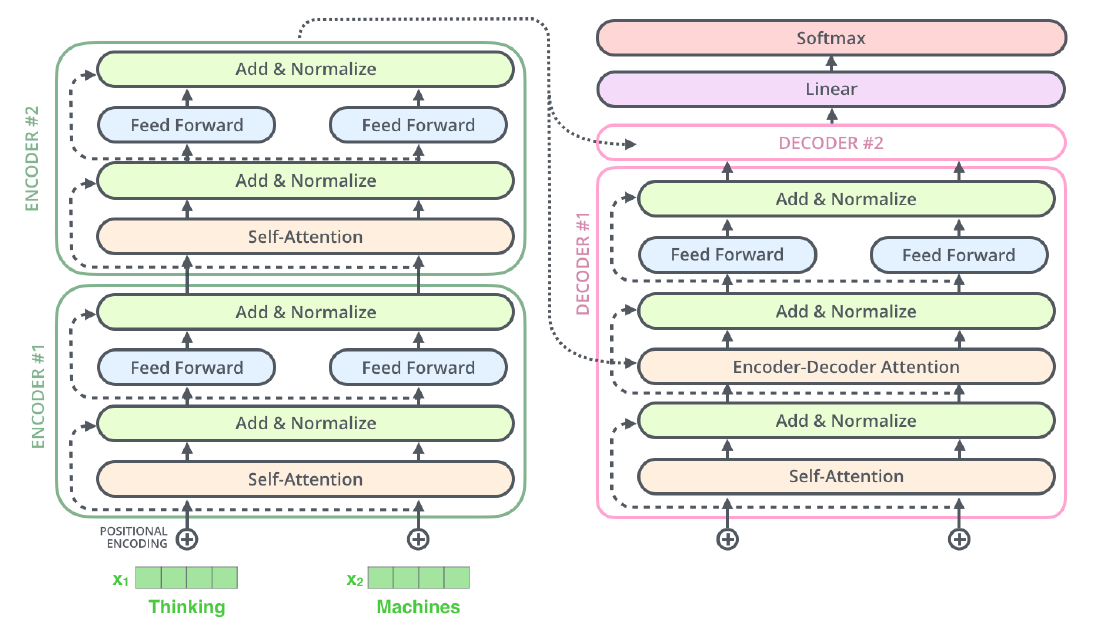
\includegraphics[width=0.75\textwidth]{transformer.png}
\end{figure}

The decoder of a Transformer is similar to the encoder, with the addition of encoder-decoder attention layers. The decoder takes a prefix of an output sentence as input and predicts the next word until it generated an \b{end token} as output. Its self-attention layer is only allowed attend to earlier predictions in the output sentence, the future positions are masked.

\subsection{Limitations of Attention}
\begin{itemize}
    \item The complexity of storing the self-attention matrix of an input of length \f{n} is \f{O(n^2)}.
    \item Attention can not deal with arbitrary long inputs. The input has to be split into segments.
    \item Low inductive bias.
    \item Need to be very large to reach good performance.
\end{itemize}

\section{Methodology}
\subsection{Batch Normalization}
\b{Problem:} Training and test data and the internal representations have different variance and mean. This leads to SGD being slow and hard to optimize. Therefore, we would like our network to normalize the data, as every batch is a different distribution that must be adaptable.\\

\b{Goal:} Make all dimensions 0-mean and unit-variance by applying:
\cf{\hat{x}^{(k)}=\frac{x^{(k)}-\mathbb{E}\left[x^{(k)}\right]}{\sqrt{\text{Var}\left[x^{(k)}\right]}}}

Batch Normalization should be applied after FC/Conv. layers and before the activation function. During testing batch norm becomes a linear operator.\\

Advantages of using batch norm:
\begin{itemize}
    \item Makes deep networks much easier to train.
    \item Improves gradient flow.
    \item Allows for higher learning rates and thus faster convergence.
    \item Networks become more robust to initialization.
    \item Acts as regularization during training.
\end{itemize}

\subsection{Layer Normalization}
In contrast to batch norm layer norm normalizes across the dimensions of the input instead of the batch size. It behaves the same for train and test.

\subsection{Transfer Learning}
Weights from self-supervised learning can be used to initialize weights for a target task. Adding classifiers or fine-tuning layers is required.\\

\b{Transfer learning methods in Vision:} Self-prediction, contrastive learning, supervised image classification, \dots\\
\b{Transfer learning methods in NLP:} Next sentence prediction, masked language modeling, \dots

\definition{\b{Meta-Learning} describes learning assumptions (inductive bias or prior) that can be transfered to new tasks.\\
It can be utilized to learn better architectures, hyperparameters, good initial weights and better loss functions.}

\subsection{Parameter Initialization}
How we choose the initial parameters affects the convergence, minimal cost and generalization error of our model.\\

\b{Current strategy:} Initialize weights for each unit separately and avoid symmetry. The weights are initialized at random following a uniform or normal distribution, the biases are initialized constant. For initializing weights, the scale is important as it could lead to gradient explosion, generalization, activation flow or symmetry breaks. We e.g. use \b{Xavier initialization}, which is a normalized initialization defined as:
\cf{W_{i,j}\sim U\left(-\sqrt{\frac{6}{m+n}}, \sqrt{\frac{6}{m+n}}\right),}
where \f{m} are the layers inputs and \f{n} the layers outputs. To compromise between goals of initializing all layers have the same activation variance and gradient variance.\\
The bias is most often set to 0, except for output units where it is set to match the desired output statistics; ReLU where it is set to 0.1 to avoid saturation; and gating units where it is set to \f{\sim 1} to open the gate.\\

\b{Other strategies:}
\begin{itemize}
    \item \b{Warm-starting:} Initialize with weights that have been optimized on a different task.
    \item \b{Meta-learning:} Learning the "best" initialization strategy for different tasks.
\end{itemize}

\subsection{CNN Architectures}
\b{U-Net:}
\begin{itemize}
    \item Consists of a contracting and expanding path.
    \item Uses up-convolution to increase the resolution after the bottleneck.
    \item Uses \f{1\times 1} convolutions in the final layer to generate the final segmentation mask.
    \item Applies data augmentations.
\end{itemize}

\b{ResNet:}
\begin{itemize}
    \item Introduces residual (identity) mappings (skip connections) around convolutional layers.
    \item Enables very deep networks.
    \item Uses batch normalization.
    \item Only one FC layer at the end.
\end{itemize}

\section{\acp{vae}}
\subsection{Autoencoders}
Autoencoders are networks that are trained to reconstruct their input. The usual architecture is something like
\cf{
\text{encoder} \to \text{bottleneck } h\to\text{decoder}
}
where the encoder encodes the input by some function into latent representation, and the decoder creates the reconstruction based on this representation. Architecture and regularization are chosen to preven simple copying. As the network learns by the discrepancy between input and reconstruction, autoencoders learn in an unsupervised fashion.

\subsection{Regularized Autoencoders}
\begin{itemize}
    \item Dimensionality \f{h \geq} dimensionality of \f{x \to} overcomplete representation
    \item Model capacity can be chosen based on the complexity of the data distribution.
    \item Prevent simple copying of the input e.g. by adding sparsity penalty on the hidden layer activations.
\end{itemize}

\subsection{Sparse Autoencoders}
\begin{itemize}
    \item Add a sparsity penalty \f{\Omega(h)} on the code \f{h} in the hidden layer to the loss function: \f{\fL + \Omega(h)}.
    \item Often used as an unsupervised pre-processing step for downstream supervised processing.
    \item Sparsity as regularization to avoid overfitting and increase generalization.
    \item Joint distribution: \f{p_{\text{model}}(x,h) = p_{\text{model}}(h)p_{\text{model}}(x|h)}
    \item We maximize: \f{\log p_{\text{model}}(x,h) = \log p_{\text{model}}(h)+\log p_{\text{model}}(x|h)}
    \item Sparsity can be implemented using a Laplace prior: \f{p_{\text{model}}(h_i) = \frac{\lambda}{2}\exp(-\lambda|h_i|),} where \f{\lambda} is a (learnable) hyperparameter
\end{itemize}

\subsection{Denoising Autoencoders}
Rather than adding an explicit regularization term, denoising autoencoders (DAE) learn to undo the effect of noise corruption when learning to reconstruct the input. To implement this, the input is corrupted by a corruption process \f{C(\tilde{x}|x)} before being fed into the encoder. The optimization is performed by the gradient descent with respect to the following negative log-likelihood. As a result, we obtain the reconstructed distribution \f{p(\tilde{x}|x)}. Note that the latent vector is deterministic in this method, but if we make it stochastic, it is equivalent to variational auto-encoder.


\subsection{\acp{vae}}
The idea behind generative models is to randomly sample from the latent space and decode to generate truly new data.\\
Assuming set of visible variables \f{x} and latent variables \f{z} our goal is to model the
distribution of the training data:
\cf{p(x)=\int p(x,z)dz = \int p(x|z)p(z)dz}
Once we have a good approximation of \f{p(x)}, we can sample from it and generate new
data that is very similar, but different from our original training data.\\

But how do we get \f{z} values that are related to our input data? This is the problem of inferring the posterior distribution \f{p(z|x)}. Since we can't use Bayes theorem to get \f{p(z|x)}, we have to resort to approximate inference methods:

\definition{Approximate inference methods approximate the posterior with a simpler distribution \f{q(z|x)} with its own set of parameters and optimize them to get as close as possible to \f{p(z|x)} by maximizing the evidence lower bound (ELBO), which minimizes the KL-Divergence.}

The \ac{vae} uses two neural networks: an encoder network with parameters \f{\phi} that learns to approximate the posterior \f{q_\phi(z|x)}, and a decoder network with parameters
\f{\theta} that learns to reconstruct the input \f{p_\theta(x|z)}. With this parametrization, the ELBO for variational inference is:
\cf{
    \fL(\theta, \phi, x) = - KL(q_\phi(z|x)\Vert p_\theta(z)) + \mathbb{E}_{q_\phi(z|x)}[\log p_\theta(x|z)]
}
where the first part is the regularization term and the second part is the reconstruction term.\\

To approximate the loss, we have to sample from posterior over \f{z}, but sampling is not a
continuous operation. To mitigate this, we can reparametrize to express our random variable \f{z} as a deterministic variable and an external, static noise source expressed in random variable \f{\epsilon}.

\begin{figure}[h!]
    \centering
    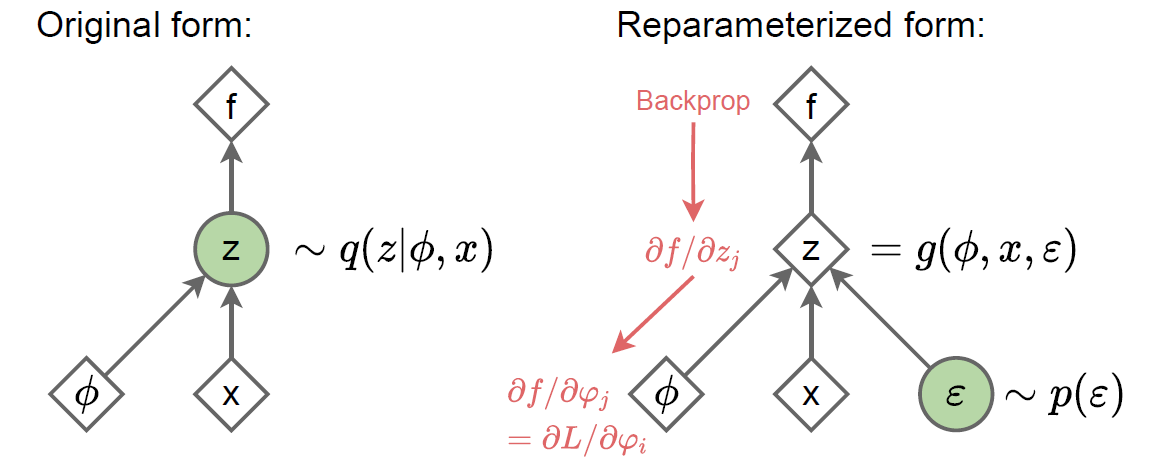
\includegraphics[width=0.6\textwidth]{reparam.png}
\end{figure}

With this reparametrization, both the decoder and the encoder can be trained together using backpropagation to optimize the ELBO.

\newpage

\section{\acp{gan}}
GANs are generative models, similar to VAEs, but drop the assumption of optimizing the lower variational bound. Hence they often produce better results.\\
\b{Idea:} We want to sample from our training distribution, but there is now way to do this. Instead, we sample from a simple distribution, e.g. random noise, and learn the transformation to training distribution.\\

GANs consist of two networks: the Generator and the Discriminator. The Generator tries to fool the discriminator by generating real-looking images. The Discriminator then tries to distinguish between real and fake images. Both networks are trained jointly in an alternating fashion. We perform gradient \b{ascent} on the discriminator and gradient descent on the generator. The most important part during training is to have a good balance between Generator and Discriminator. It can easily happen that one outperforms/underperforms the other. After training, the generator can be used to generate new images.

\subsection{Diffusion Models}
Denoising diffusion models consist of two processes:
\begin{enumerate}
    \item Forward diffusion process gradually adds noise to input data by sampling from a Gaussian \f{T} times.
    \item Reverse denoising process generates output by denoising.
\end{enumerate}

The forward diffusion process is a Markov process that leads to the joint probability:
\cf{
    q(x_{1:T}|x_0) = \prod_{t=1}^{T}q(x_t|x_{t-1}) 
}
The schedule of the noise is designed such that \f{q(x_T|x_0)\approx\mathcal{N}(x_T; 0,1)}.\\

The denoising process starts by sampling \f{x_t\sim q(x_T)\approx\mathcal{N}(x_T;0,1)} and then iteratively sampling \f{x_{t-1}\sim q(x_{t-1}|x_t)}. Even though this is generally intractable, we can approximate this with a Gaussian if \f{\beta_t} is small enough. This means that we can learn the mean of a Gaussian to approximate \cf{q(x_{t-1}|x_t) \approx \mathcal{N}(x_{t-1};\mu_\theta(x_t,t),\sigma_t^2I),} where \f{\mu_\theta(x_t,t)} is the trainable network.

\begin{figure}[h!]
    \centering
    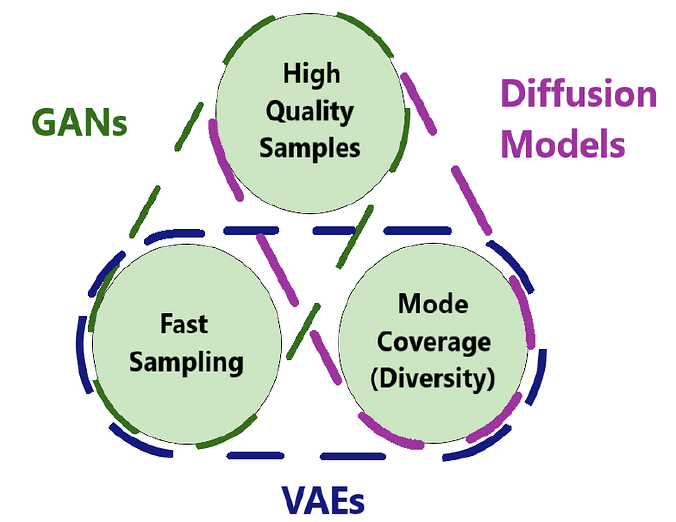
\includegraphics[width=0.4\textwidth]{gen.png}
\end{figure}

\section{Uncertainty Estimation}
Knowing model's uncertainty is crucial in safety-critical applications such as medical diagnosis, autonomous driving, etc. The output probability (softmax) of standard neural networks is typically not reliable. For example, deep neural nets can be overconfident for unrecognizable images. In these cases, the uncertainty should grow away from the typical data seen, but it doesn't.\\
For regression NNs, the uncertainty should look something like the following:
\begin{figure}[h!]
    \centering
    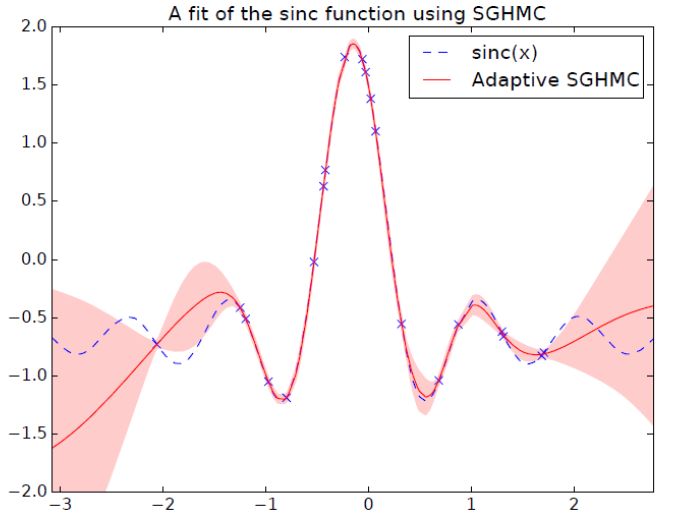
\includegraphics[width=0.5\textwidth]{uncertain.png}
\end{figure}

There are several types of uncertainty:
\begin{enumerate}
    \item \b{Aleatoric:} Intrinsic observation (data) noise.
    \item \b{Epistemic:} Uncertainty about the model, can be reduced by more data.
\end{enumerate}

\definition{Being Bayesian about NNs means dealing will all sources of parameter uncertainty: As more than one weight vector can explain the observed data, we need to take into account all possible explanations.}

\subsection{DNGO Model}
The DNGO model aims at being Bayesian at least about the output layer. DNGO first trains a neural network on a given dataset and use the feature vector obtained in the last hidden layer as basis functions of the Bayesian linear regression.

\subsection{Bayesian Neural Networks}
Given data \f{\mathcal{D}=(X,y)}, parameters \f{\theta}, a prior distribution \f{p(\theta)} and a likelihood \f{p(y|X, \theta)}, the core part of Bayesian Neural Networks is to compute the posterior distribution:
\cf{
    p(\theta|\mathcal{D}) = p(\theta|X,y) = \frac{p(y|X,\theta)p(\theta)}{p(y|X)} = \frac{p(y|X,\theta)p(\theta)}{\int p(y|X,\theta)p(\theta)d\theta}
}
\b{Problem:} Since the mean of \f{p(y|X,\theta)} is not a linear function of \f{\theta} and Gaussians are not closed under non-linear mappings, the posterior is not a Gaussian anymore. Approximating the posterior requires variational inference or the  Markov-Chain-Monte-Carlo method.

\subsection{Variational Inference}
Variational Inference (VI) is an optimization-based method for approximating intractable probability distributions in Bayesian inference. Instead of directly computing a complex posterior distribution \( p(z \mid x) \), VI approximates it with a simpler distribution \( q(z \mid \lambda) \) by minimizing the Kullback-Leibler (KL) divergence:
\[
q^*(z) = \arg\min_{q \in \mathcal{Q}} D_{\text{KL}}(q(z \mid \lambda) \parallel p(z \mid x)).
\]
This converts Bayesian inference into an optimization problem, making it computationally feasible for high-dimensional models.\\
In order to minimize this KL-Divergence w.r.t to \f{\theta}, we only need to maximize the ELBO. ELBO embodies a trade-off between satisfying the complexity of the data and satisfying the simplicity of the prior. ELBO is very popular since it approximates the true posterior with the variational posterior and therefore replaces the diffcult integral.

\subsection{Markov-Chain-Monte-Carlo (MCMC) Method}
Another posterior estimation is performed by MCMC. MCMC samples each weights according to a
proposal distribution or transition distribution \f{p(w_{t+1}|w_t)} and moves around the space while accepting or rejecting the proposal from the distribution. Since the next state is determined only by the current state, it is called Markov-chain. For the nal sampling, we use every \f{t}-th sample from the history to avoid the correlation between samples close to each other in terms of time steps. The goal of the sampling is to identify the stationary distribution \f{\pi} that is ideally the posterior distribution
\f{p(w|\mathcal{D})}. The sufficient condition for a stationary distribution to exist is that the detailed balance \f{\pi(w_t)p(w_{t+1}|w_t)=\pi(w_{t+1})p(w_t|w_{t+1})}. In practice, even when the detailed balance is satisfied, it may still take time to reach the stationary distribution. This time (from the beginning) is called mixing time. Intuitively, the distribution reaches the stationary distribution when the chain forgets the beginning states. Therefore, we take samples after a burning-in phase and the length of the burn-in phase is a hyperparameter.


\subsection{Prior-Fitted Networks (PFNs)}
PFNs are neural networks trained to approximate Bayesian inference by learning a prior distribution over possible data-generating processes. Instead of traditional training on a fixed dataset, PFNs are trained on a diverse set of synthetic tasks sampled from a prior, enabling them to generalize to new tasks without gradient-based fine-tuning. This allows PFNs to perform rapid adaptation in a Bayesian manner while leveraging neural network expressiveness.\\
PFNs might be a disruptive alternative to variational inference and MCMC.


\subsection{Output Ensembling}
Construct an ensemble of \f{M} neural networks on the training data. For each test data point \f{x} predict with each of the \f{M} networks and combine the outputs to obtain probabilistic predictions:
\cf{
    f(x) = \frac{1}{M}\sum_{i=1}^{M}f_i(x),\quad\text{(classification case)}
}
where \f{f_i(x)} is the output of the \f{i}-th network. For the regression case we can compute the empirical mean and variance across the predictions like so:
\cf{
    \mu_x = \frac{1}{M}\sum_{i=1}^{M}f_i(x)
}
\cf{
    \sigma_x^2 = \frac{1}{M}\sum_{i=1}^{M}(f_i(x)-\mu_x)^2
}

The \f{M}-Ensemble can be created in different ways: via dropout (simply by sampling \f{M} dropout masks), via MCMC, via different random seeds for SGD initialization, etc.

\subsection{The Estimation of Parametric Models}
We can train a network with weight \f{\theta} to output the parameters \f{w} of a parametric model \f{p(y|x,w)}. Most commonly we have the network output \f{\mu} and \f{\log(\sigma^2)} of a Gaussian \f{\mathcal{N}(\mu, \sigma^2)}.\\
This can be achieved by simply maximizing the log-likelihood w.r.t. network weight \f{\theta}:
\cf{
    \log p(\mathcal{D}|\theta) = \frac{1}{N}\sum_{i=1}^{N}\log p(y_i|w(x_i, \theta)).
}
The predictive distribution for an input \f{x} is then defined as:
\cf{
    p(y|x,\theta) = p(y|w(x,\theta)).
}
These predictive uncertainties can then be combined with ensembling. Each network \f{i} with weights \f{\theta_i} predicts a probability distribution with mean \f{\mu_{x,i}} and variance \f{\sigma_{x,i}^2}.\\
We can combine these predictions in a mixture distribution, using the law of total variance to compute the mean \f{\mu_x} and variance \f{\sigma_x^2} as:
\cf{
    \mu_x = \frac{1}{M}\sum_{i=1}^{M}\mu_{x,i}
}
\cf{
    \sigma_x^2  = \frac{1}{M}\sum_{i=1}^{M}\left((\mu_{x,i}-\mu_x)^2+\sigma_{x,i}^2\right)
}

\section{AutoML / \ac{hpo}}
Neural networks are very sensitive to many hyperparameters, e.g.:
\begin{itemize}
    \item Optimization: SGD variant, lr-schedule, momentum, batchsize, \dots
    \item Regularization: dropout rates, weight decay, data augmentation, \dots
\end{itemize}

\definition{
    Let \f{\theta} be the hyperparameters of an ML algorithm \f{\mathcal{A}} with domain \f{\Theta}, \f{\mathcal{D}_{opt}} be a training set which is split into training and validation split and \f{\mathcal{L}(\mathcal{A}_\theta, \mathcal{D}_{train}, \mathcal{D}_{val})} denote the loss of \f{\mathcal{A}_\theta} trained on \f{\mathcal{D}_{train}} and evaluated on \f{\mathcal{D}_{val}}.\\
    The HPO problem is to find a hyperparameter configuration which minimizes the loss:
    \cf{
        \theta^*\in\arg\min_{\theta\in\Theta}\fL(\mathcal{A}_\theta, \mathcal{D}_{train}, \mathcal{D}_{val})
    }
}
Hyperparameters can have different types, such as numerical (continuous, integer) or categorial (boolean, categories e.g. choice of optimizer). Additionally, some hyperparams are only active if other hyperparams take certain values. Furthermore, some hyperparams (learning rate) naturally lay on a logarithmic scale. Tuning all these parameters manually could be a tedious task.

\subsection{Practical Tips}
In general, HPO is useless unless the model can overfit the training dataset. For this reason, one good strategy is to make sure that the model (i.e. training loss) can overfit the subset and then move tothe HPO of validation loss on the full dataset. As another tip, the learning rate is typically important, so one heuristic is to increase learning rate until the loss diverges and then reduce it a little bit.

\subsection{Black-Box Optimization}
Black-box optimization is to optimize functions without derivative information. The most basic algorithm is random search and it maintains global search and can be computed in parallel. Additionally, it can deal with low intrinsic dimensionality compared to grid search. Another famous example is local search and it fixes the best configuration and changes the configuration along only a single axis.

\subsection{Bayesian Optimization}
\b{General approach:}
\begin{itemize}
    \item Fit a probabilistic model to the collection functions samples
    \item Use the model to guide optimization, trading off exploration vs exploitation
\end{itemize}

\subsection{Population-based Methods}
Uses a population of configurations and the "survival of the fittest" principle. Based on evolutionary strategies.

\subsection{HPO Speedup Techniques}
There are several techniques to speed up black-box HPO optimization:
\begin{enumerate}
    \item \b{Meta-Learning:} Follows the idea of learning about learning methods by optimizing the performance of known learning methods and generating new ones, transferring the learned knowledge in the process.
    \item \b{Extrapolating of learning curves:} Terminate learning curves that are not promising.
    \item \b{Multi-Fidelity optimization:} Using iterative ML algorithms, poor runs can be stopped early. Using k-fold cross-validation, poor hyperparam settings can be rejected after a few folds. Bad models can be ruled out based on their performance on data subsets.
\end{enumerate}

\b{Successive Halving:}
\begin{itemize}
    \item Try different configurations and drop the worst ones after a certain time.
    \item Next, drop the next generation after double the time. Repeat.
    \item Problem: Some configurations might be bad in the beginning but good in the end.
\end{itemize}

\b{Hyperband:}
\begin{itemize}
    \item Same as successive halving, but takes different time budgets as lowest fidelity.
    \item This is done without taking already tested settings into account.
\end{itemize}

\b{BOHB:}
\begin{itemize}
    \item Uses Bayesian optimization for choosing configurations.
    \item Uses Hyperband for selecting the budgets.
\end{itemize}

\subsection{Combining User Beliefs with Bayesian Optimization}
Prior user knowledge could be helpful for selecting well-performing hyperparameter configurations.\\

\b{PriorBand:}
\begin{itemize}
    \item Combines user priors with multi-fidelity optimization
    \item Uses three different configuration sampling schemes: random, user prior over location of good configurations, loccaly around incumbent
    \item Less uniform random configurations for higher fidelities
    \item Over time, give higher weight to strategies that were more successful in this run
    \item Advantage: Even performs well (in the long run) if given a bad prior
\end{itemize}

\subsection{Hyperparameter Gradient Descent}
Let \f{\fL_{val}(w,\theta)} denote the validation loss of a network with weights \f{w} and
hyperparameters \f{\theta}; likewise, \f{\fL_{train}(w,\theta)} is the training loss.\\
Then, the optimization of \f{\theta} can be written as the following bilevel optimization problem:
\cf{
    \min_\theta\fL_{val}(w^*(\theta),\theta)
}
\cf{
    s.t.\quad w^*(\theta)\in\arg\min_w\fL_{train}(w,\theta)
}
This enables us to compute gradients for \f{\theta} by differentiating through the entire SGD optimization run that leads to \f{w^*(\theta)}. Weight and hyperparameter optimization steps can then be interleaved (does not guarantee convergence).

\subsection{Neural Architecture Search (NAS)}
NAS aims to automatically optimize architectural choices, making it a special case of HPO. NAS also allows for special speedup techniques: sharing \& inheriting weights.\\
All possible architectures are subgraphs of a large supergraph: the one-shot model. Weights are shared between different architectures with common edges in the supergraph. Search costs are reduced drastically since one only has to train a single model.\\

\b{DARTS:} Use one-shot model with continuous architecture weight \f{\alpha} for each operator. By optimizing the architecture weights, DARTS assigns importance to each operation. And since \f{\alpha} is continuous, we can optimze them with gradient descent. In the end, DARTS discretizes to obtain a single architecture.\\

\b{Weight Entanglement:} Weight entanglement reduces memory complexity of the supernet by reusing weights, not only between architectures that share the same operation (i.e. edge in the graph) but also between operations.\\

\b{Weight Inheritance:} When locally expanding a network (e.g., adding a layer), we can inherit the weights of the unchanged part, which avoids costly retraining of the unchanged part. The newly introduced weights can be initialized to yield a \b{network morphism} (operators that change the network structure, but not the modelled function).

\end{document}
